% Simulation: computing the VIX from option quotes (Nikita).

\subsection{Computing the VIX from option quotes}
\subsubsection{Data}

We took a snapshot of S\&P~500 index options from Yahoo Finance (15-minute delayed quotes) on \textbf{5 November 2026 at 11:41 ET}, together with the S\&P~500 level (7,476.22) and the official VIX at the same moment (22.54). The snapshot contains 2,118 SPXW options across ten expirations between 27 November and 11 December 2026; 97.8\% have a positive bid. Risk-free rates are the 1- and 3-month constant-maturity Treasury yields from the US Treasury daily par yield curve (4.01\% and 4.21\% on 4 November 2026).

\subsubsection{Implementation}

The calculation (\texttt{vix\_calc.py}) follows the Cboe methodology \cite{cboemeth}:
\begin{enumerate}
  \item \textbf{Expirations.} Select the first two Friday expirations more than 23 and fewer than 37 days away. Standard third-Friday SPX options settle at 9:30 ET; weekly SPXW options settle at 16:00 ET. Time to expiry is measured in minutes, $T=M/525{,}600$.
  \item \textbf{Rates.} Interpolate the 1-month (30-day) and 3-month (91-day) Treasury yields linearly to each expiry, then convert each from a bond-equivalent yield (BEY) to a continuously compounded rate, as Cboe does:
  \[ \mathrm{APY}=\left(1+\tfrac{\mathrm{BEY}}{2}\right)^2-1, \qquad R=\ln(1+\mathrm{APY}). \]
  \item \textbf{Forward and $K_0$.} Use mid-quotes; find $K^*$ minimising $|C-P|$, compute $F$ from \eqref{eq:cboe}, and take $K_0$ as the first strike at or below $F$.
  \item \textbf{Strike selection.} Out-of-the-money puts below $K_0$ and calls above $K_0$, skipping zero bids and stopping after two consecutive zero bids; the average of put and call at $K_0$.
  \item \textbf{Variance and interpolation.} Apply \eqref{eq:cboe} to each expiry and \eqref{eq:interp} to obtain the 30-day VIX.
\end{enumerate}

\subsubsection{Validation against Cboe's worked example}

Before using live data, we ran the same code on the option data in Appendix~1 of the Cboe VIX White Paper \cite{cboewp} (186 near-term and 128 next-term strikes, extracted from the PDF text), with Cboe's stated inputs ($T$ in minutes, $R_1=0.0305\%$, $R_2=0.0286\%$). Table~\ref{tab:cboe} shows that every intermediate quantity matches.

\begin{table}[H]
\centering
\small
\begin{tabular}{@{}lrr@{}}
\toprule
\textbf{Quantity} & \textbf{Our code} & \textbf{Cboe}\\
\midrule
$T_1$ & 0.06834855 & 0.0683486\\
$T_2$ & 0.08826865 & 0.0882686\\
$F_1$ & 1962.89996 & 1962.89996\\
$F_2$ & 1962.40006 & 1962.40006\\
$K_0$ (both terms) & 1960 & 1960\\
$\sigma_1^2$ & 0.01846292 & 0.01846292\\
$\sigma_2^2$ & 0.01882101 & 0.01882101\\
VIX & 13.685821 & 13.685821\\
\bottomrule
\end{tabular}
\caption{Our implementation on Cboe's worked example. The only differences are in $T$, where Cboe rounds to seven decimals. Because $\sigma^2$ depends on every selected strike, the match also confirms that the code selects exactly the same strikes as Cboe.}
\label{tab:cboe}
\end{table}

\subsubsection{Live result: 5 November 2026}
\label{sec:live}

\begin{table}[H]
\centering
\small
\begin{tabular}{@{}lrr@{}}
\toprule
 & \textbf{Near term} & \textbf{Next term}\\
\midrule
Expiry (SPXW, 16:00 ET) & Fri 4 Dec 2026 & Fri 11 Dec 2026\\
Minutes to settlement & 42,018 (29.18 days) & 52,098 (36.18 days)\\
$T$ (years) & 0.079944 & 0.099122\\
$R$ (continuous) & 0.039703 & 0.039902\\
$K^*$ & 7,500 & 7,500\\
Forward $F$ & 7,498.0438 & 7,501.4055\\
$K_0$ & 7,490 & 7,500\\
Strikes used (puts / $K_0$ / calls) & 89 / 1 / 87 & 51 / 1 / 54\\
Strike range & 3,200--8,700 & 3,200--9,000\\
$\sigma^2$ (volatility) & 0.050506 (22.47\%) & 0.050951 (22.57\%)\\
30-day weight & 0.8828 & 0.1172\\
\midrule
\textbf{Calculated VIX} & \multicolumn{2}{r}{\textbf{22.49}}\\
\textbf{Official VIX} & \multicolumn{2}{r}{\textbf{22.54}}\\
\textbf{Difference} & \multicolumn{2}{r}{$-0.05$ points}\\
\bottomrule
\end{tabular}
\caption{VIX computed from the 5 November 2026 snapshot.}
\label{tab:live}
\end{table}

The calculated VIX is within 0.05 points (0.2\%) of the official value. The remaining gap comes from inputs rather than the formula: Cboe interpolates rates with a cubic spline across the whole Treasury curve while we use two points; the option quotes and the official value were recorded seconds apart and are delayed; and Cboe's real-time quote feed and filtering differ from Yahoo's quotes.

A VIX of 22.5 means the market expects S\&P~500 volatility of about 22.5\% a year, or roughly $\pm 22.5/\sqrt{12}\approx\pm6.5\%$ over the next 30 days. The previous day the VIX closed at 16.61 with the S\&P~500 at 7,688.62; by the snapshot the index had fallen 2.8\% and the VIX had risen by 5.9 points, the ``fear gauge'' behaviour described in the discussion section.

\begin{figure}[H]
  \centering
  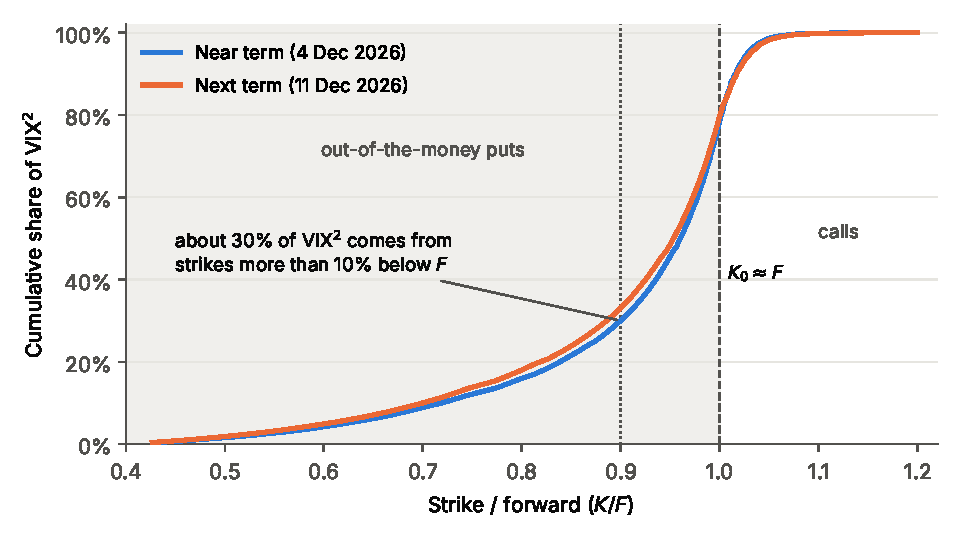
\includegraphics[width=0.85\linewidth]{figures/vix_strike_contributions.pdf}
  \caption{Cumulative share of $\sigma^2$ by strike, 5 November 2026 snapshot. About 76\% of the variance comes from out-of-the-money puts and 22\% from calls; roughly 30\% comes from puts more than 10\% below the forward.}
  \label{fig:contrib}
\end{figure}

Figure~\ref{fig:contrib} shows how the variance is built up across strikes. Puts supply about three quarters of VIX$^2$, and nearly a third comes from strikes more than 10\% below the forward. This is the combined effect of the $1/K^2$ weights and the skew: deep out-of-the-money puts are expensive because investors pay for crash protection. The VIX is therefore largely a price of crash insurance, which is why it rises sharply when the market falls.

\subsubsection{Numerical verification of the replication}

To confirm \eqref{eq:result} independently of Cboe's data, \texttt{verify\_variance\_replication.py} applies \eqref{eq:cboe} to option prices from two models in which the expected variance is known exactly. All prices use a forward of 100, $T=30/365$ and $r=4\%$.

\begin{table}[H]
\centering
\small
\begin{tabular}{@{}lrr@{}}
\toprule
\textbf{Strike grid} & \textbf{Strip variance} & \textbf{Volatility}\\
\midrule
Fine and wide (step 0.05, 20--300) & 0.040001 & 20.000\%\\
SPX-like spacing and range (step 0.07, 43--120) & 0.039997 & 19.999\%\\
Narrow range only (90--110) & 0.039056 & 19.763\%\\
Very coarse spacing only (step 5) & 0.045066 & 21.229\%\\
\bottomrule
\end{tabular}
\caption{Black--Scholes with $\sigma=20\%$ (true variance 0.04). The strip recovers the true variance; truncating the strike range lowers it and very coarse spacing raises it, as in Table~\ref{tab:assumptions}. A step of 0.07 at a forward of 100 matches SPX's 5-point spacing at 7,500.}
\label{tab:bs}
\end{table}

\begin{table}[H]
\centering
\small
\begin{tabular}{@{}lrr@{}}
\toprule
\textbf{Heston model, 200{,}000 Monte Carlo paths} & \textbf{Variance} & \textbf{Volatility}\\
\midrule
Exact expected variance $\theta+(v_0-\theta)\frac{1-e^{-\kappa T}}{\kappa T}$ & 0.028010 & 16.736\%\\
Simulated average realised variance & 0.028025 & 16.741\%\\
Option strip with $1/K^2$ weights & 0.028025 & 16.741\%\\
\bottomrule
\end{tabular}
\caption{Under Heston (parameters from \cite{gatheral}: $\kappa=1.3253$, $\theta=0.0354$, $\sigma=0.3877$, $\rho=-0.7165$; $v_0=0.0276=(16.61/100)^2$, the VIX close on 4 November 2026; full-truncation Euler, 24 steps per day), option prices are Monte Carlo averages over the same paths. The strip is within 0.1 standard errors of the exact value although volatility is random.}
\label{tab:heston}
\end{table}

Together, Tables~\ref{tab:cboe}--\ref{tab:heston} show that the formula is implemented correctly, that it reproduces the official index on live data, and that it recovers expected variance in a stochastic-volatility model, as the derivation predicts.
